\chapter{Compression on the basis of equivalence classes}

\section{Related Compression Techniques}
Compression of high-throughput sequencing reads becomes crucial with the lowering cost of sequencing technology. The rapid technological development enables the generation of petabytes of data on servers worldwide. Apart from size, often succinct representation \citep{Pritt2016} can yield very similar results with a much smaller memory footprint. Nucleotide sequence compression can largely be divided into two paradigms, one is reference-based compression, where the reference must be transferred to the decoder along with the compressed data ~\citep{Canovas2014}, \citep{Fritz2011}, \citep{Li2014}. Another is reference-free compression, \citep{adjeroh2002dna},\citep{Bonfield_2014}, \citep{Hach2012} where the read sequences are compressed independent of reference sequence, eliminating the burden of transferring a reference. Such compressions are commonly known as \Denovo compression. A robust and recently-introduced \denovo compressor, LEON \citep{Benoit2015}, constructs a probabilistic de Bruijn graph from the k-mer counts table built on the reads. Reads are then mapped to the newly constructed de Bruijn graph, and are stored in the form of an anchor address, the read size, and bifurcation list.   

Reference-based compressors typically start with BAM files produced by state-of-the-art aligners such as \Bowtie. One serious bottleneck of reference based compression, is to store all the meta-information in the BAM file which can be regenerated by re-aligning the reads to the provided reference sequence. This problem can be easily solved storing the edits after aligning the sequences to reference. \citet{Fritz2011} introduced one such widely used tool \texttt{mzip} which can store alignments permitting users to avoid compressing quality score, unaligned sequences. \texttt{fastqz} \citep{bonfield2013compression} bypassed the problem of storing meta data by implementing a new alignment technique.

\begin{figure}[!ht]
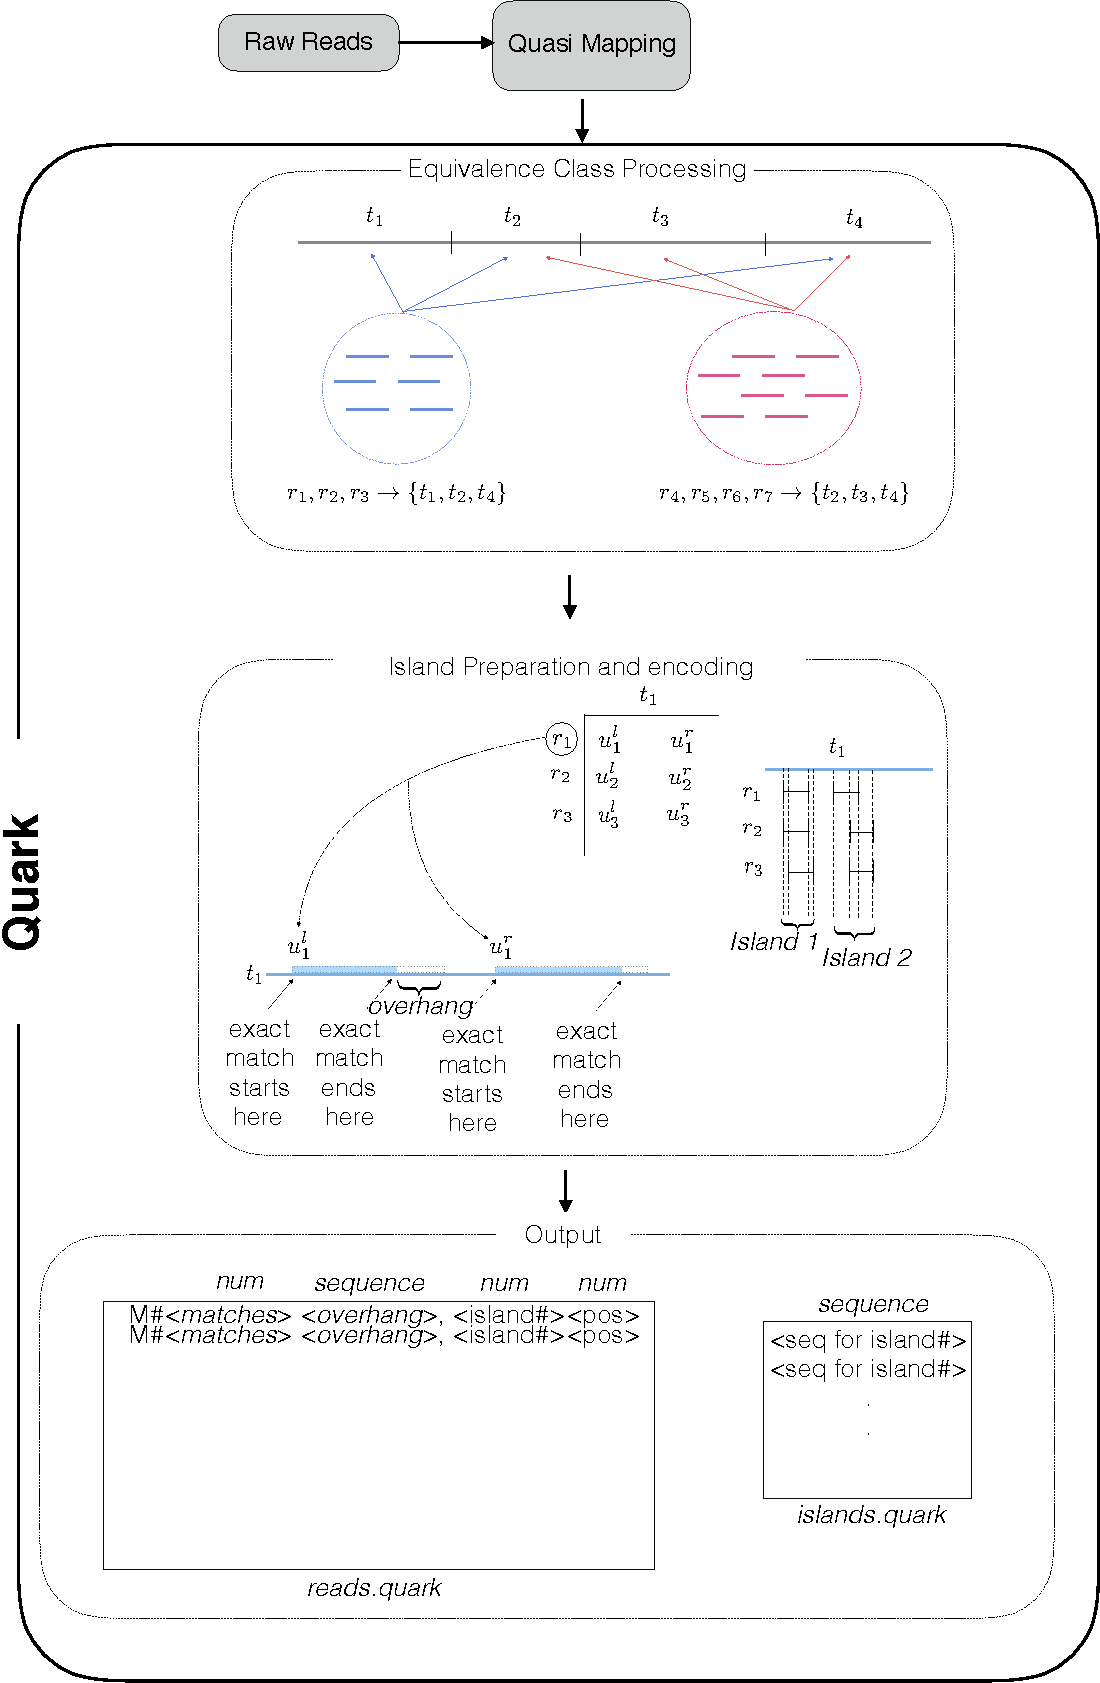
\includegraphics[width=\textwidth]{Figures/quark_overview4-crop}
\centering
\caption{\label{fig:overview_quark}An overview of the \quark pipeline. Equivalence classes are computed using \qm. Reads within classes along with the positions are then used find out the exact match length and the overhang portion. Islands are simultaneously processed from the intervals. In the last steps, encoded reads along with the islands are stored as \quark output.}
\end{figure}


The recently-published CORA ~\citep{Yorukoglu2016} is a compressive read mapper. The working principle of CORA is interesting and worth mentioning as concept of equivalence classes is also used there, but carries a different meaning. CORA converts the fastq reads to non-redundent k-mer sets. Furthermore, CORA does a redundancy removal on reference genome, by performing self-mapping. The positions where a k-mer maps form an equivalence class. Two equivalence classes are regarded as concordant if all positions of one equivalence class are in one nucleotide shift distance from another equivalence class. 

Apart from reference-based and \denovo tools, some methods lie in the middle.  For example, Kpath \citep{Kingsford2015} is a tool that assumes a k-mer distribution given by a reference transcriptome, and compresses the reads by grouping them together by their starting k-mers and encoding them as arithmetically coded paths in a de Bruijn graph.  In this case, the reference k-mer distribution acts as a backbone for a statistical generative model and primes the arithmetic coder.

In the current chapter we present a semi-reference-based compression tool, \quark, which takes the raw reads and transcripts from the user and perform a \qm on it. The mapping information is then utilized to represent the reads. The motivation for such a scheme comes from the observation of the fact that a small fraction of the transcriptome is often sufficient to represent the vast majority of mapping reads in an experiment, and therefore, storing the entire transcriptome is often unnecessary. A decoder on the other end takes the small subset of the transcriptome sequence, that we refer to as \iss, and the compressed reads to produce the uncompressed data. An overview of \quark is given in \fref{fig:overview_quark}. The method section is divided into three parts, in the heart of \quark, \qm maps the raw reads to the indexed transcriptome and reports the position of the read (anchored by a series of right-maximal exact matches). In the next step, we collect the position and the target transcripts, and subsequently merge the reference sequences overlapping the mappings to yield a set of \iss. We describe the method in greater detail in \sref{sec:quark_method}

\section{Method}\label{sec:quark_method}
At a conceptual level \quark exploits the mapping principle used in \qm, therefore it is worth going over the basic mechanism of \qm adopted from \citet{rapmap}. In \fref{fig:overview_quasi} the basic steps of \qm is described. \Qm starts with a matched \kmer that is shared between a transcript and read sequence. If such a match exists, \qm tries to extend the match further by searching the interval of the suffix array for a maximum mappable prefix. The match is used to determine the \textit{next informative position} in the reference sequences, and the same mapping process continues from that point within the query.

 
\begin{figure}[!ht]
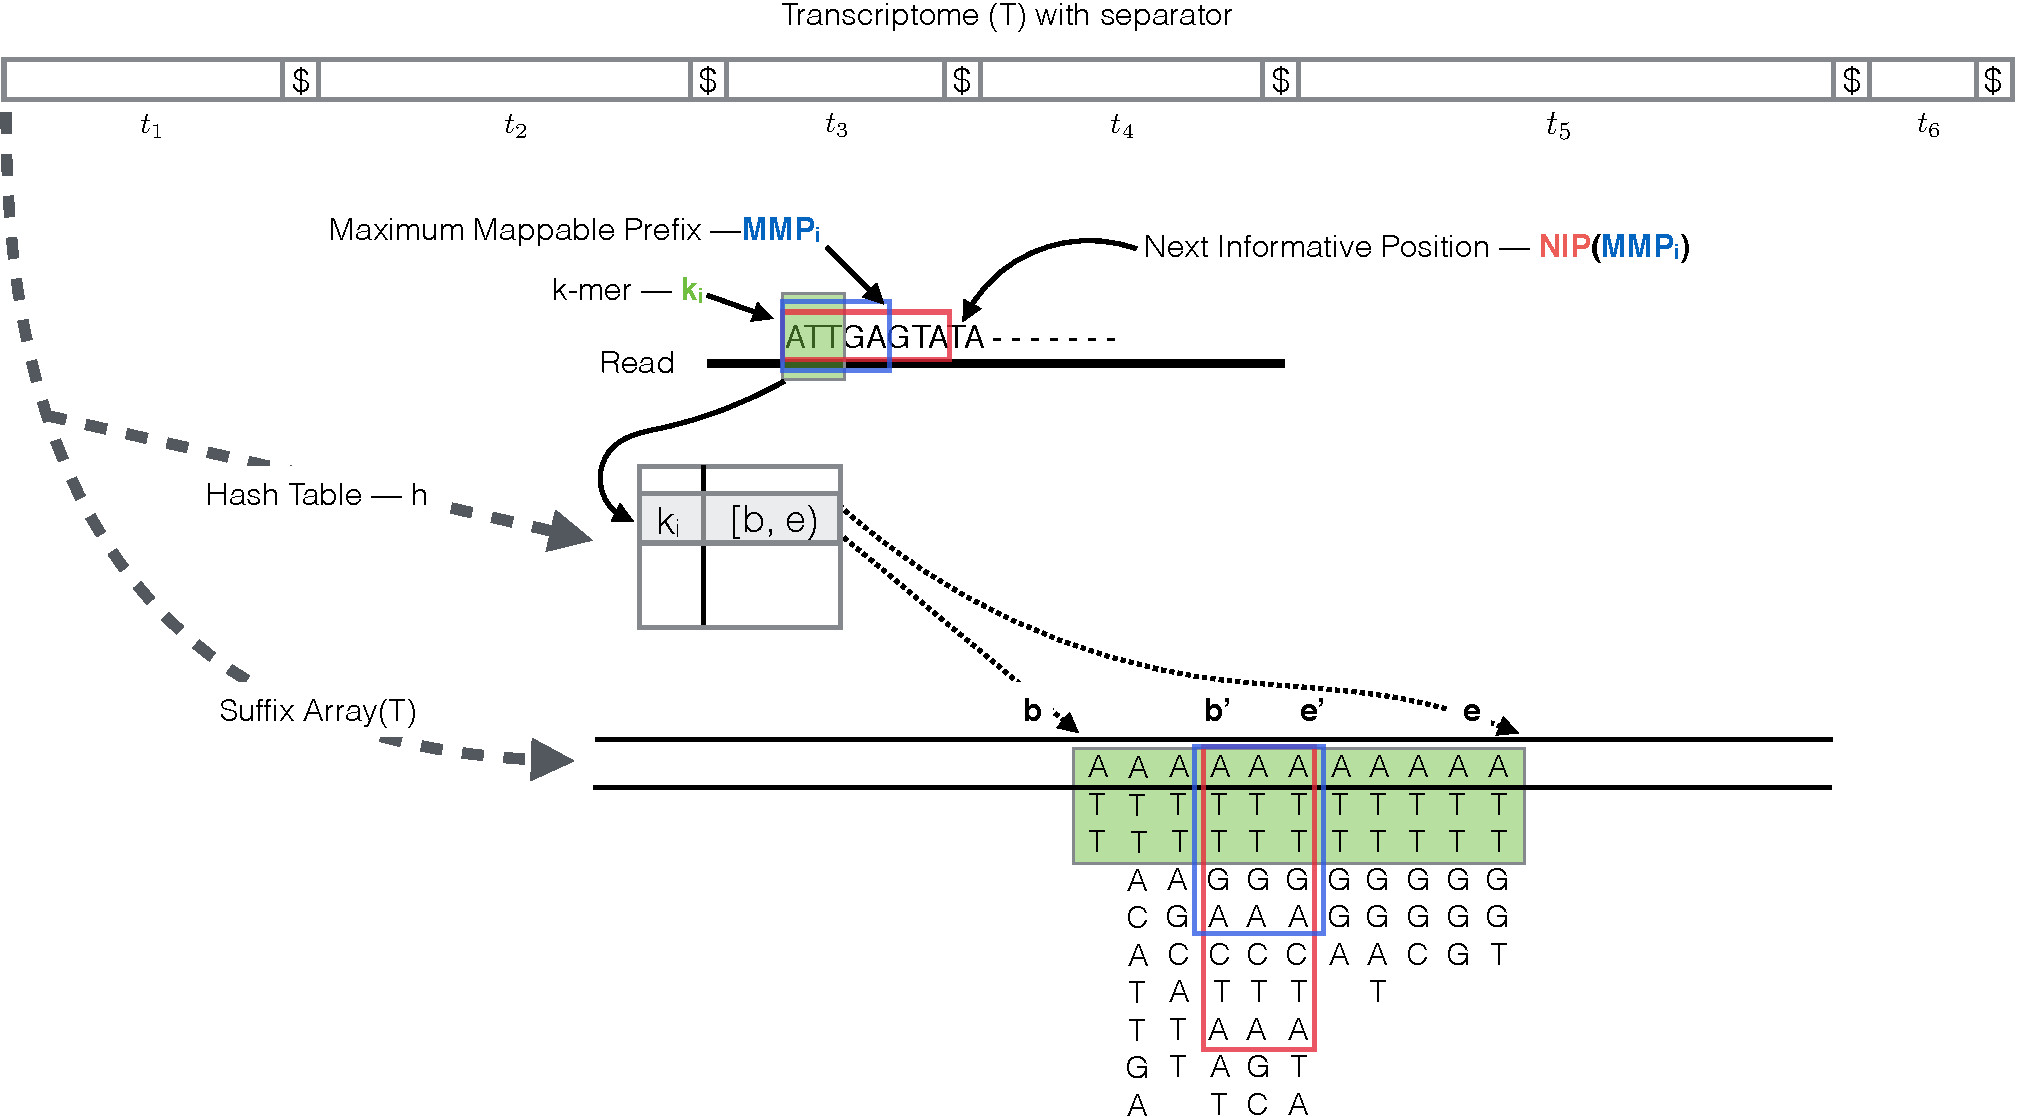
\includegraphics[width=\textwidth]{Figures/overview_quasi}
\centering
\caption{\label{fig:overview_quasi}The transcriptome (consisting of transcripts $t_1,\ldots ,t_6$) is converted into a $\$$-separated string, $T$, upon which a suffix array of T, and a hash table, $h$, are constructed. The mapping operation begins with a \kmer (here, $k=3$) mapping to an interval $\{b,e\}$ in suffix array of T.}
\end{figure}

We divide the \textit{quasi-mapped} reads into three categories, 
\begin{itemize}
    \item {\it Mapped reads:} If both the reads of the mate pair are mapped. This is an ideal situation where we can encode both the ends efficiently. Because each of the reads shares some sequence with the reference.
    \item {\it Orphan reads:} For reads in this category we can not map both ends of the mate pair. In \quark we encode the unmapped end directly.
    \item {\it Unmapped reads:} There is no mapping at all for the read, as determined by the \qm algorithm, and so the read is instead encoded using a reference-free approach.
\end{itemize}

Given the above results, in \quark, we follow a hierarchical structure, where the mapped reads are distributed into equivalence classes according to \sref{subsec:gen_equiv_classes}. Knowing the fact that all reads in equivalence classes share a right-maximial exact match with the reference transcript and each other. The encoding scheme itself is straight forward. Given the position and the reference sequence, we do a linear search on the reference sequence to find out the maximal match. This search is guaranteed to yield a match of at least $31$ nucleotides given the criterion of \qm.

\subsection{Island Construction}

Formation of \iss are very similar to what we see in certain assembly methods. Given the intervals on the reference sequence that might share some nucleotides, we merge the intervals to form disjoint \iss. As shown in \fref{fig:overview_quark} the encoded reads are assigned to an \is id. The use of \is aids the compression abilities of \quark, and additionally makes the resulting compression file self-contained, eliminating the need to assume the decoder has access to the saem reference. To study the effectiveness of constructing \iss, we considered dataset SRR635193. After mapping to the Gencode reference transcriptome for human, we observe that out of 95,309 transcripts, only 49,589 transcripts are used by \quark. Moreover as shown in \fref{fig:ratio}, there are a lot of transcripts where only a small fraction of nucleotides participate in islands.  

\begin{figure}[!ht]
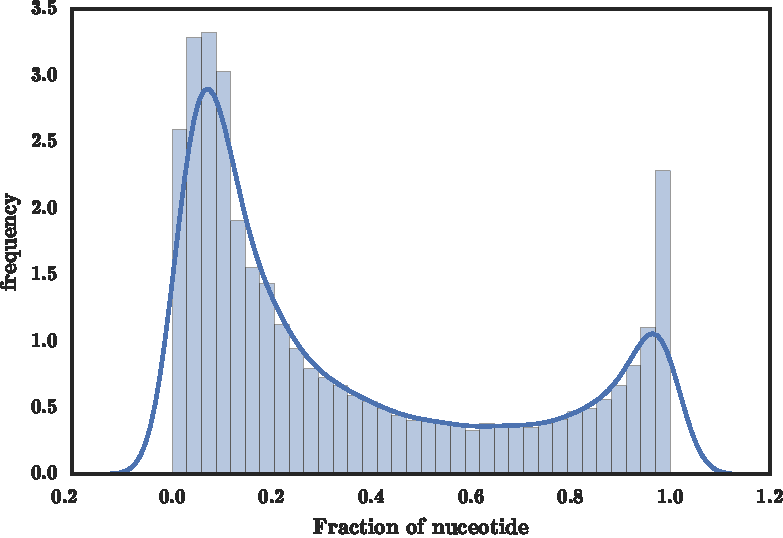
\includegraphics[width=0.5\textwidth]{Figures/ratio}
\centering
\caption{\label{fig:ratio}Islands consist of only a fraction of nucleotides of expressed transcripts}
\end{figure}

\subsection{Post-processing}
As a post processing step, we further use \texttt{lzip} to compress \textit{read.quark} and \textit{islands.quark} files, which contain the encoded reads and the sequences of the islands, respectively. As the size of the unmapped reads can not be improved by \qm, we use off-the-shelf \denovo compression tool \texttt{SCALCE} \citep{Hach2012} to compress these reads. 

\section{Results}
We tested our approach with real data from SRR635193, SRR445718 and SRR490961. The compressed sequence size is presented in \tref{tab:performance_table}. In terms of size on disk \quark out performs both \texttt{leon} and \texttt{SCALCE}. 

\begin{table}
\caption{Size of the read files after compression along with raw \texttt{fastq} gzipped size (bytes)}
\centering
\begin{tabular}{lrrrr}
\toprule
{} &     \texttt{fq.gz}  &    \quark &     \texttt{leon} & \texttt{SCALCE} \\
\midrule
SRR635193 & 2,329,761,348    &     \bf{140,069,396}     &      384,918,555 & 294,962,419 \\
SRR445718 & 2,848,487,774    &     \bf{171,723,783}     &    328,915,302  &  253,352,974\\
SRR490961 & 4,115,142,514    &     \bf{203,458,347}     & 466,622,492 & 301,777,076 \\
\bottomrule
\end{tabular}
\label{tab:performance_table}
\end{table}

